
\section{Architettura del Sistema}

\subsection{System Boundary}

In figura~\ref{fig:system-boundary} viene illustrata la divisione del sistema di HBS in sottosistemi, e i rapporti che intercorrono fra i sottosistemi e i sistemi esterni ad HBS.
Una descrizione dettagliata degli elementi presenti in figura~\ref{fig:system-boundary} viene fornita nelle sezioni seguenti.

\begin{figure*}[h]
	\centering
	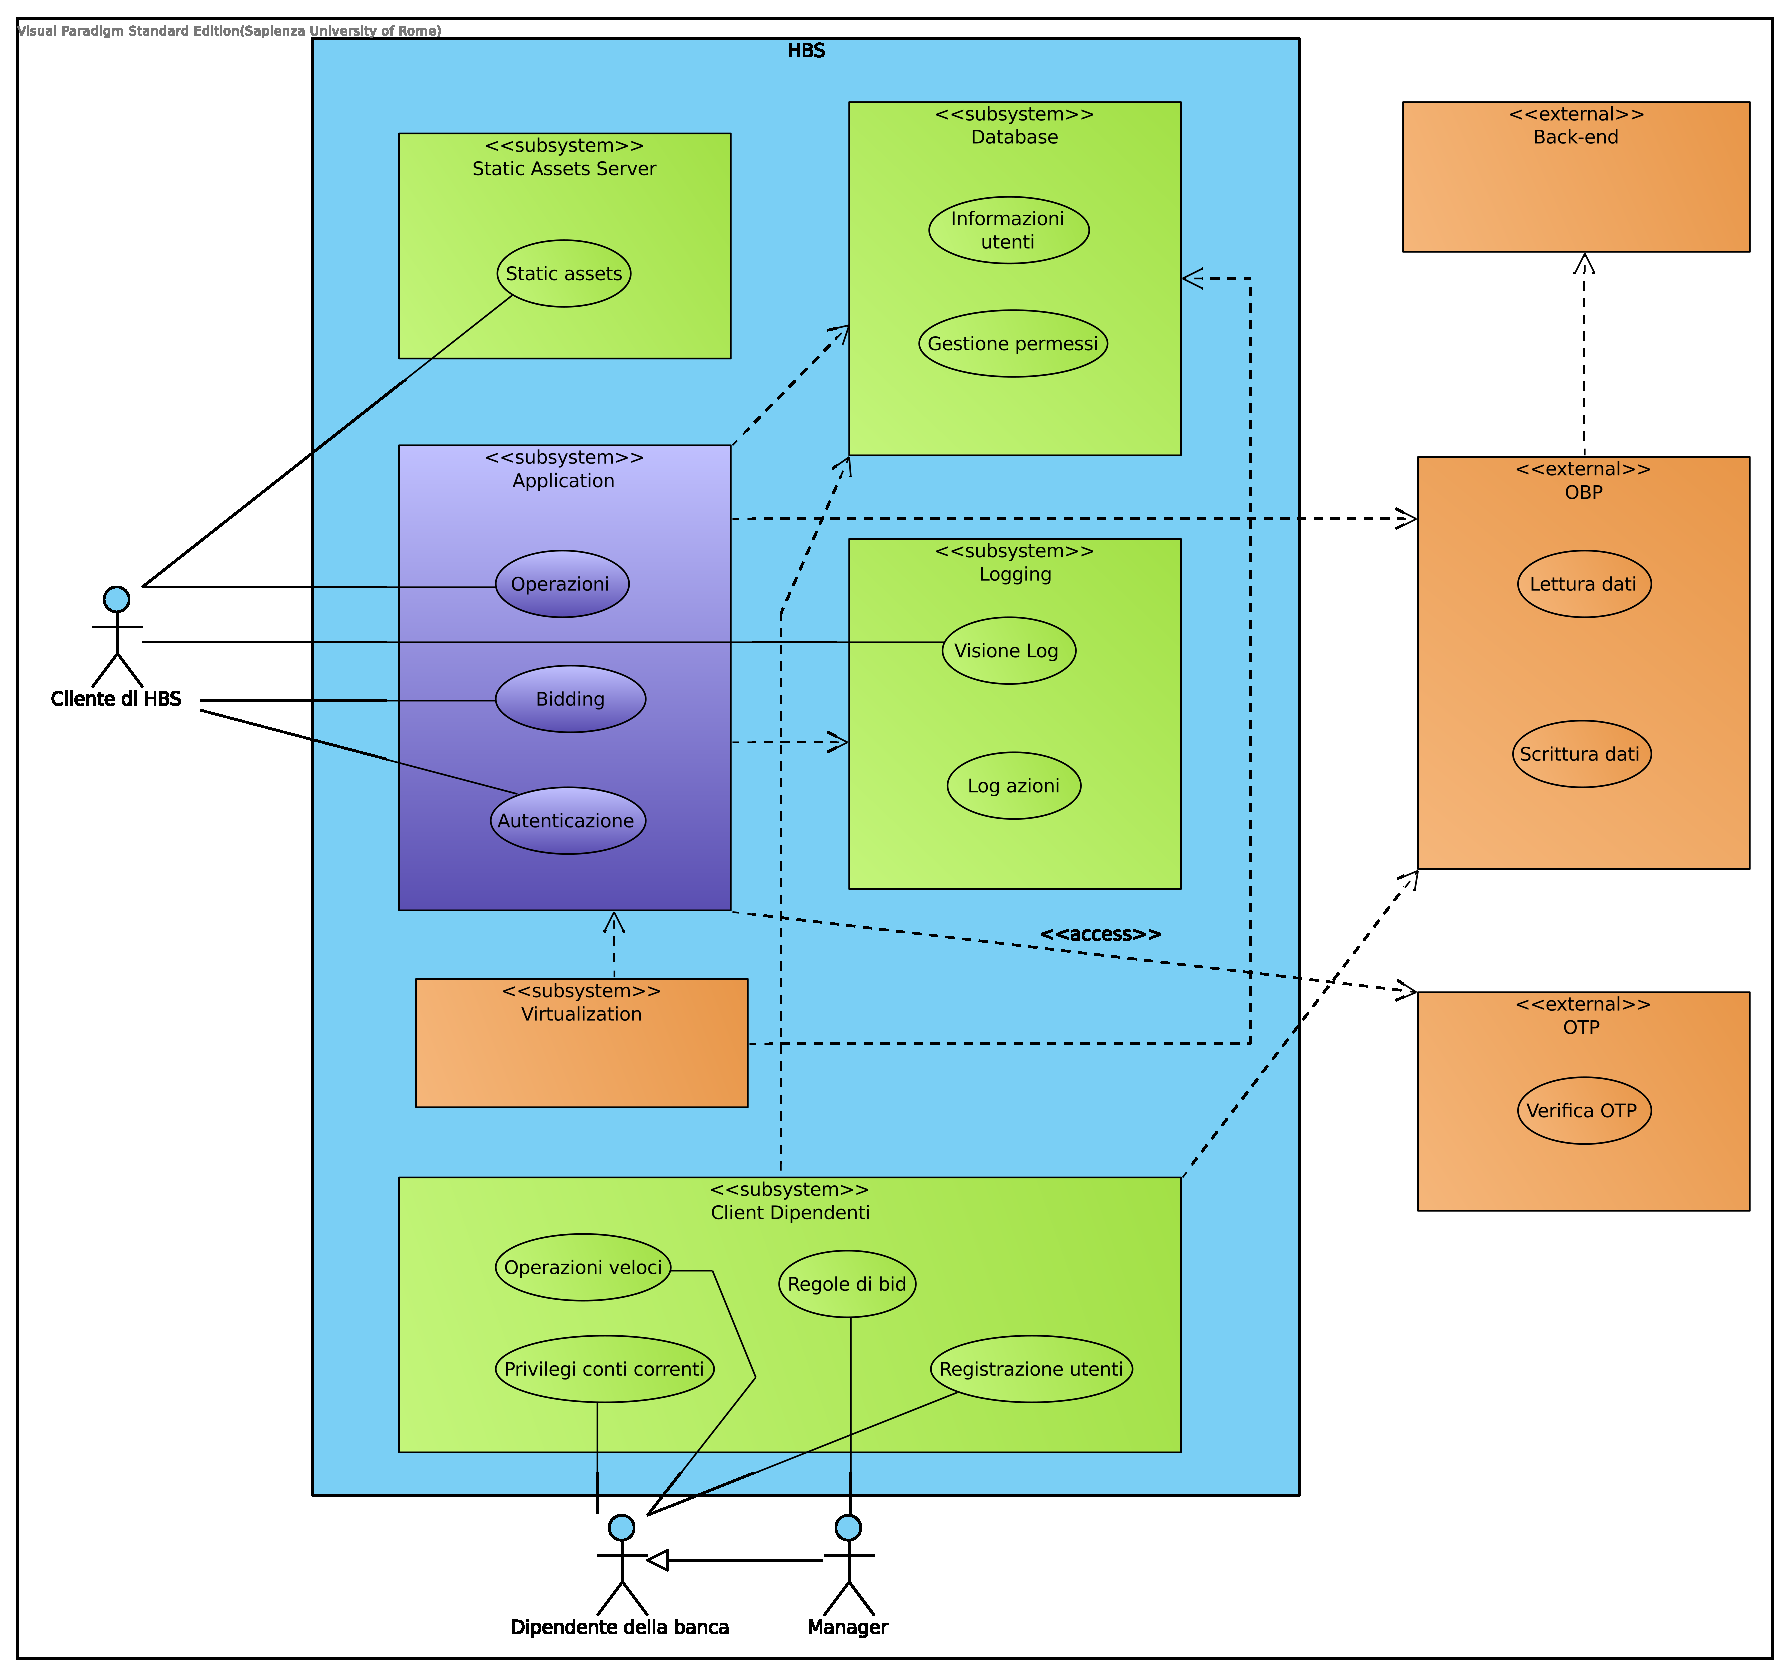
\includegraphics[width=\textwidth]{Images/System_Boundary.eps}
	\caption{Architettura del sistema.}
	\label{fig:system-boundary}
\end{figure*}

\subsection{Virtualization Master}
Questa componente logica comunica con tutti i master, ed \`e la responsabile della virtualizzazione.
Consiste di un software di controllo di virtualizzazione e si occupa di far partire e spegnere le istanze.
Inoltre mantiene la lista di istanze attive.
In caso di riavvio di un master esso deve richiedere la lista delle istanze dal Virtualization Master, per dopo fare polling di ogni singola istanza per dedurre lo stato attuale del sistema.
Questa componente esiste al di fuori di una macchina virtuale e ne controlla il comportamento.
Il malfunzionamento di Virtualization Master ha conseguenze gravi sul sistema, questa componente del sistema deve essere fault tollerant.
\subsection{Static Data}

Questo sottosistema serve per fornire ai clienti l'accesso ai file statici, come immaggini e fogli di stile.

\subsubsection{Assets Server}
I server di questo gruppo sono semplici server HTTP. Sono raggiungibili da Internet all'indirizzo static.hbs.***.**. Questi server non contengono dati personali degli utenti oppure informazioni riservarte della banca, per questo non \`e necessario l'utilizzo dei protocolli sicuri come HTTPS.
\`E necessaria anche una componente software che monitora il carico su ogni singolo server e comunica questi dati allo Static Master.
Il paradigma di distribuzione adottato in questo sottosistema \`e duplicazione, ogni server \`e una copia esatta dell'altro.
I server static data non inviano informazioni al sistema di logging, ogni server mantiene un log locale per motivi di debug e sicurezza, ma i log vengono cancellati periodicamente.
Per effettuare le modifiche ai dati contenuti bisogna effettuare la stessa modifica su tutti i server.
\subsubsection{Static Master}
Lo static master raccoglie i dati dai singoli server, ed effettua il \emph{load balancing} fra i server.
Aggiorna molto frequentemente il \emph{server dns}, in modo che risponda alla richiesta del nome static.hbs.***.** con l'indirizzo ip del \emph{Assets Server} meno occupato.
%TODO glossario DNS
In caso non ci siano istanze sufficienti per processare tutte le richieste degli utenti con latenza accettabile, il master si occupa di avviare nuove istanze di \emph{Assets servers}.
In caso ci siano uno o pi\'u \emph{Assets servers} che sono inattivi perch\'e non ci sono abbastanza richieste, il master disattiva alcune istanze.
In caso di malfunzionamento di un server \`e sufficiente rimuovere il suo indirizzo dalla lista dei server, in modo che il DNS non dia pi\`u il suo indirizzo agli utenti finch\`e non viene ripristinato.
In caso di malfunzionamento di Static Master il sistema rimane in funzione, ma potrebbe avere un calo di prestazioni.
Per ripristinare il funzionamento basta avviare un altra istanza di Static Master.
\subsection{Application}

\subsubsection{Application Server}
Sono server HTTP che processano le richieste degli utenti e generano dinamicamente i contenuti.
Sono raggiungibili da Internet all'indirizzo hbs.***.** .
Il traffico dati di questi server comprende informazioni sensibili come password ed informazioni personali degli utenti, per questo bisogna forzare l'utilizzo del protocollo HTTPS.

Il software HTTP comunica con il software HBS tramite il protocollo \emph{CGI} - Common Gateway Interface.
I server di questo gruppo inviano informazioni al sistema di logging, in particolare a ogni operazione rilevante bisogna salvare dati relativi nel log.
Ogni application server viene eseguto indipendentemente dagli altri senza comunicazione, inoltre non contengono dati, solo software.
In caso di malfunzionamento di un server \`e sufficiente rimuovere il suo indirizzo dalla lista dei server, in modo che il DNS non dia pi\`u il suo indirizzo agli utenti finch\`e non viene ripristinato.
%TODO glossario CGI
Il software HBS comunica con il DB master, preleva la mappa di partizionamento per accedere ai singoli DB server.
\subsubsection{Application Master}
L'application master raccoglie i dati riguardo al carico dai singoli server, per poter effettuare \emph{load balancing}.

Aggiorna molto frequentemente il \emph{server dns}, in modo che risponda alla richiesta del nome hbs.***.** con l'indirizzo ip del \emph{Application Server} meno occupato.
%TODO glossario DNS
In caso non ci siano istanze sufficienti per processare tutte le richieste degli utenti con latenza accettabile, il master invia una richiesta al Virtualizzation Master per avviare nuove istanze di \emph{Application servers}.
In caso ci siano uno o pi\'u \emph{Application servers} che sono inattivi perch\'e non ci sono abbastanza richieste, il master disattiva analogamente alcune istanze.
Il master comunica con il sistema di logging.
L'istante esatto di avvio e spegnimento di ogni istanza viene salvato nel log.

In caso di malfunzionamento di un server \`e sufficiente rimuovere il suo indirizzo dalla lista dei server, in modo che il DNS non dia pi\`u il suo indirizzo agli utenti finch\`e non viene ripristinato.
Ogni malfunzionamento deve essere comunicato al sistema di logging.
In caso di malfunzionamento di application master il sistema rimane in funzione, ma le performance possono ridursi signitificativamente, non possono essere avviate e disattivate istanze di application server.

\subsection{Database}
\subsubsection{DB server}
I server di questo gruppo sono sistemi database che vengono utilizzati per memorizzare informazioni.% . . .
Per distribuire il carico ed assicurare la consistenza dei dati la politica di distribuzione dell'informazione che si usa \`e \emph{Range partitioning}, ovvero le informazioni vengono partizionate in base al valore dell'identificatore, e ogni sistema mantiene un range di valori.
Non ci sono informazioni condivise fra istanze distinte e le istanze non comunicano, questo facilita la consistenza ma potrebbe diminuire la \emph{Fault tollerance} del sistema, per questo bisogna assicurarsi che l'hadware di storaggio dati sottostante \`e ridondante come in caso di RAID5.
In caso di malfunzionamento di un server, un range di utenti non potra accedere al sistema.
%possiamo dire che usiamo anche duplicazione cioe ogni server ha anche un istanza mirror, cosi se va giu non va giu il sistema
%mettiamo questo come modifica apportata cosi sembra che abbiamo trovato un problema e l'abbiamo risolto quanto siamo belli
%ogni server ha un server mirror che duplica tutti i contenuti e ogni modifica deve essere apportata anche al server mirror, ogni transazione per essere committed deve necessariamente completare anche sul database mirror.
%Questo forza la consistenza.
%In caso di malfunzionamento di un server succede questo:
%application server fa richiesta ad un db ma non riceve risposta, fa richiesta al db master, il db master verifica che il db server sia effettivamente morto, db master risponde al appserver guarda quello \`e chioppato usa il backup,dice al backup che \`e da solo e non ha un backup , db master manda un  sms all'admin guarda coglione che ti \`e chioppato un server pirla, il db master si ricorda che il db server \`e morto e non riverifica piu, aggiorna la mappa della partizione con backup server come primario
%quando riparano/rimpiazzano il server rotto devono rimettere in ordine il database, facciamo che il software db sa farlo da solo,
% il server ripristinato diventa il backup e quello attivo rimane primario
% lo si comunica al db master, ed db master configura il server attivo a forzare le modifiche sul nuovo backup, facciamo che \`e una procedura unica ``copia modifiche che ti sei perso e diventa backup''
%allora diventa
%Ogni server ha 3 modalit\`a di funzionamento:
%\begin{itemize}
%\item Primario - il server \`e il primario: riceve le richieste dagli app server; se sono delle query risponde, se sono delle modifiche prima le fa sul proprio database poi le propaga sul backup, se fallisce su uno dei due fa rollback.
%\item Primario senza backup
%\item Backup - il backup funziona come \emph{mirror} e non deve rispondere alle query.

\subsubsection{DB master}
Il master raccoglie le informazioni dai singoli server, ma non effettua il \emph{load balancing} dinamicamente.
Aiuta a individuare i server che non sono in grado di garantire i tempi di risposta accettabili, ma l'introduzione di una nuova istanza del DB server comporta un cambiamento alla mappa della partizione. \`E un lavoro \emph{batch} che comporta l'indisponibilit\`a temporanea dei server interessati, e per ci\`o va fatto solo su richiesta dell'amministratore di sistema.

Il DB master mantiene la mappa della partizione aggiornata, e la fornisce su richiesta del Application Server.
Ogni cambiamento della mappa viene comunicato al Sistema di Logging.
In caso di malfunzionamento di DB master la mappa della partizione non sar\`a disponibile, il sistema rimane in funzione ma le nuove istanze di application server non possono essere avviate.
Ogni funzionamento anomalo di un DB server deve essere registrato nel log.
\subsection{Servizio Autenticazione}
\subsection{OTP Server}
\`E una macchina dedicata ad elaborare le richieste OTP. Richiede il seguente software:
\begin{itemize}
    \item Client NTP - per tenere aggiornato l'orologio di sistema.
        %TODO gigi scivi come se ci manomettono l'orologgio di questa  macchina possono accedere con otp vecchi e for soldi in soldi battono soldi
    \item Un DBMS per mantenere i seed OTP.
    \item Un software OTP per validare la risposta OTP dell'utente.
%Single point of failure su sto povero server
%possiamo fare sta grande mossa e dire che ce ne siamo accorti mamma mia
%e diciamo che mettiamo un backup anche a sto server
\end{itemize}

\subsection{Servizio Logging}
\subsubsection{Sistema di logging}
Questa \`e una componente logica del sistema.
Corrisponde al servizio di routing del DBMS NOSQL sottostante.
Riceve richieste dalle altre componenti del sistema e le esegue sul database.
Il software DBMS si occupa del partizionamento e distibuzione dei dati.
Si sceglie questa tipologia di DBMS perch\'e \`e pi\`u adatta ai sistemi distribuiti.

\subsubsection{Server Logging}
Ogni istanza di questo gruppo esegue un DBMS NOSQL, ovvero database non relazionale.
In questo caso si sceglie un database orientato ai documenti che permette la distribuzione \emph{Sharded} dei dati.
%TODO glossario sharded https://docs.mongodb.com/manual/core/distributed-queries/

